% CREATED BY DAVID FRISK, 2016
\chapter{Model}
The simulation is at the essence a particle-based model. Spherical particles are used to represent entities analogous to biological cells, both dead and living, as well as energy particles. This chapter will describe the simulation model, including the physics implemented to handle the particle interactions and the evolutionary and organism-related structures created around them.


\section{Particle-based physics}
Each particle has properties such as position, velocity, force, radius, density and energy level, which are accessible and modifiable in the concurrent interaction functions. Particles also have a given particle type and, if their particle type is \emph{Cell}, also a given cell type.

\subsection{Interaction functions}
Functions that need to be applied to a majority of particles, such as handling terrain collisions, boundary conditions, buoyancy, energy decay and position updates, are implemented as interaction functions and are executed in parallel on the GPU through the Fluidix library.

This is also true for particle-pair interactions: For all non-buffer particles within a predefined distance, a repulsive force is applied unless they are cell neighbours (see Figure \ref{fig:neighbours}). Depending on the particle types (and for cells also their cell types) energy will be exchanged between the particles upon contact. For example, a digestive cell colliding with an detritus particle will some of its energy.

Finally, the model also made use of particle-to-surface interactions to handle collisions between particles and the terrain described in subsection \ref{subsec:terrain}. 

\subsection{Particle types} \label{subsec:particleTypes}
There are four particle types implemented in the model: \emph{Cells}, \emph{Detritus}, \emph{Buffer} and \emph{Energy particles}. Particles change type depending on what happens to them in the simulation and transform according to Figure \ref{fig:particleCycle}. The number of particles might be decreased if there exists an excess number of buffer particles at the end of the particle array, but the normal action for an unneeded particle is to turn into a buffer particle.
\begin{description}
    \item [Cell] The cell particle is analogous to the biological cell, although a significant simplification. Apart from the ordinary particle properties, a cell also has knowledge of which organism it belongs to (by an organism ID), which cells are its neighbours, and what type of cell it is. Neighbouring cells will, while in contact, exchange energy with each other, where the amount being exchanged depends on the cell types (see Table \ref{tab:cellEnergies}).
    \item [Detritus] When a cell has less energy than the predefined amount \emph{minCellEnergy}, the cell dies and turns into a detritus particle. All detritus are dead cells but they might have an energy amount larger than \emph{minCellEnergy} if it died of other causes than energy deprivation. Over time, the detritus decays, losing energy, until none is left and the particle disappears (turns into a buffer particle).
    \item [Buffer particle] A limitation with the Fluidix library is that changing the number of particles is a costly operation. Because of this, the model keeps a particle buffer in order to ensure that there always will be particles available. The ones not currently in use are set as buffer particles and positioned outside the simulation boundaries. 
    \item [Energy particle] Photosynthetic cells receive energy while they have a clear path to the ceiling above them. To check if they do, energy particles are sent straight up from the photosynthetic cells to check for collisions.
    %In order to provide energy to the system, the model includes energy particles constantly falling down from the sky. Each particle contains a predefined amount of energy, which upon contact with a photosynthetic cell gets transferred to the cell while the energy particle turns into a buffer particle.
\end{description}
\begin{figure}
  \centering
  \includegraphics[width=0.3\textwidth]{"figure/particle cycle"}
  \caption{Transformations between the different particle types. Since changing the total number of particles is computationally costly, especially decreasing the particle count, a buffer is kept for creating new cell and energy particles. A cell usually turns into a detritus particle as it loses its energy, however it might in some cases turn directly into a buffer particle. Energy particles are created corresponding to the amount of photosynthetic cells and will turn into buffer particles as their respective cells die.
  }
  \label{fig:particleCycle}
\end{figure}

\subsection{Cell types} \label{subsec:cellTypes}
For cell particles another particle called cell type is also used. Cells each belong to one of eight discrete cell types, introduced to give evolution different adaptive options for harvesting and handling energy. Some cell types gain energy by interacting with other particles, while others store, transmit or simply spend energy.
\begin{description}
    \item [Photosynthetic cell] Inspired by biological photosynthesis, the photosynthetic cell receives energy while it has a clear view to the top of the simulated volume (accomplished by the use of energy particles).
    %Inspired by biological photosynthesis, the photosynthetic cell receives the energy from an energy particle upon collision.
    \item [Digestive cell] %https://en.wikipedia.org/wiki/Phagocytosis Detrivore?
    The digestive cell instead gains energy by consuming detritus (dead cells), receiving their energy upon collision.
    \item [Sting cell] %https://en.wikipedia.org/wiki/Pinocytosis ?
    While the digestive cell consumes detritus, the sting cell "steals" energy from living cells of other organisms upon contact. Both digestive and sting cells are inspired by biological phagocytes.
    \item [Vascular cell] Whereas photosynthetic, digestive and sting cells all collect energy for the organisms, the fat, sensor and egg cells only consume (and/or store) energy. The vascular cell is implemented in order to transport energy between non-adjacent cells.
    \item [Fat cell] The fat cell works as energy storage (battery). It can store more energy than the other cell types (except eggs) and has a much higher energy inflow than outflow.
    \item [Sensor cell] In order for the nervous system (described in \ref{subsec:nervousSystem}) to have any input from the surrounding world, the model includes a sensor cell. The sensor cell does not collect energy in any way, nor does it store it. However, it does observe the particles in it's vicinity and sums their energy readings into a signal value. That signal is then used as one of possible inputs to the nervous system.
    \item [Buoyancy cell] Buoyancy cells have a significantly lower density than the other cell types, allowing them to float upwards. 
    \item [Egg cell] Last, but not least, is the egg cell. An egg cell, like the fat cell, stores energy. Differing from the fat cell however, it does not have any energy outflow at all. Furthermore, the egg cell can store orders of magnitude more energy than the other cell types and it will continue to collect energy from its neighbouring cells until it has enough energy to form a new organism, in which case it immediately does.
\end{description}

\section{The arena}
This section will describe the environment created for the organisms to develop and adapt in. In order to create a non-homogeneous environment for the organisms, terrain and water was added to the model. Figure \ref{fig:arena} and Figure \ref{fig:boundaries} both shows the arena used in the final simulation described in Chapter \ref{cpt:Results}, illustrating water and terrain as well as particles and boundaries respectively.

\subsection{Water and air}
A basic implementation of water was introduced, where the density of the surrounding medium would be higher in the lower half of the simulation volume. The organisms, in normal configurations, have densities slightly higher than the water so that they with some movement effort can stay afloat, but need to spend significantly more energy to fly. The water level is exemplified together with the terrain in figure \ref{fig:arena}, where the tiny dot of the initial organism is about to fall through the air and down to bottom below the water surface.

\subsection{Terrain}\label{subsec:terrain}
The terrain collision is implemented as a particle-to-surface interaction function in the Fluidix library. Each cell or detritus particle inside the 3d terrain volume will be moved back to the closest position on the terrain surface and will experience a ground repulsive force proportional to the distance it had penetrated. As can be seen in Figure \ref{fig:boundaries}, the particles remain on the outside of the volume defined by the larger blue terrain vertices.

\begin{figure}
  \begin{center}
  \includegraphics[width=\textwidth]{figure/arena}
  \caption{
    Depiction of the arena terrain and water. These elements were introduced to enable organisms to settle in different environments and possibly diversify. The image is rendered at the initiation of the simulation described in Chapter \ref{cpt:Results}, with the single initial organism barely visible in the centre of the arena.
  }
  \label{fig:arena}
  \end{center}
\end{figure}

\begin{figure}
  \centering
  \includegraphics[width=\textwidth]{figure/boundaries}
  \caption{Visualisation of all elements of the particle model. The purple object is the terrain, with the larger blue particles making up its vertices. The multicoloured particles above the terrain are energy, detritus and cell particles, with their colour representing their energy level. The opaque particles are the cells, while the transparent particles above are mostly energy particles. A blue energy particle belongs to an occluded photosynthetic cell while a red one indicates that it has not yet collided with anything before reaching the top. Detritus particles of varying remaining energy can be seen among the organisms beneath the water surface. The thin blue bounding box determines the boundary that the particles cannot pass. The large number of blue transparent particles beneath the terrain are buffer particles.}
  \label{fig:boundaries} 
\end{figure}

\subsection{Boundaries}
The boundaries of the simulation volume, affecting cells and detritus particles, are implemented as linear soft-wall repulsion. Particles straying outside the simulation area will experience a repulsive force proportional to the trespassed distance. The boundaries can be distinguished as the thin blue edges in Figure \ref{fig:boundaries}, with the particles remaining strictly on the inside (the light-green box instead encloses the terrain particle set).

\section{Artificial genome}
Similar to biological life, this artificial life model has a genome with a genotype-to-phenotype encoding. The choice of encoding is not trivial, as it will influence how mutations traverse the space of possible phenotypes. The approach taken with this model is inspired by a method called CPPN-NEAT proposed by \cite{stanley2007compositional} which produces phenotypes using pattern-producing networks, over time mutated in their topology by a certain set of mutations. This section will detail how the method was implemented for this project.

\subsection{Compositional Pattern Producing Networks} \label{subsec:CPPN}
The encoding method CPPN, Compositional Pattern Producing Networks, is an abstraction of natural development proposed by \cite{stanley2007compositional}. They differ from previous developmental encodings in that they does not require either local interactions or temporal unfolding, but instead achieves similar properties by using a structure very similar to artificial neural networks.

Given coordinates as input, the network produces output used to set the properties of that specific coordinate. Each link in the network has a certain weight \(w\) and each node has a certain activation function \(f\). 
The activation functions implemented are the following:
\begin{description}
    \item[Sine] \includegraphics[align=c, width=30pt]{figure/activationFunctions/sine} \(f(x) = sin(x)\)
    \item[Abs] \includegraphics[align=c, width=30pt]{figure/activationFunctions/abs}\(f(x) = 1- abs(x)\), clamped within \([-1,1]\)
    \item[Id] \includegraphics[align=c, width=30pt]{figure/activationFunctions/id}\(f(x) = x\), clamped within \([-1,1]\)
    \item[Gaus] \includegraphics[align=c, width=30pt]{figure/activationFunctions/gaus}\(f(x) = e^{\frac{x^2}{2}}\)
    \item[Mod] \includegraphics[align=c, width=30pt]{figure/activationFunctions/mod}\(f(x) = x \bmod 1\)
\end{description}
The \emph{Sine} and \emph{Mod} functions contributes with repetition while the \emph{Abs} and \emph{Gaus} provide symmetry.

Values are propagated through the network by calculating the next value \(v_{i,t+1}\) of each node as its activation function of the sum of the previous values times weights for all its connected nodes; that is \(v_{i,t+1}=\sum_{j\in n}f(v_{j,t}*w_{ij})\), where \(n\) is the set of nodes connected to node i. A number of outputs is generated for any given location, resulting in a pattern. An example of this can be seen in Figure \ref{fig:cppn}.

\begin{figure}[H]
  \centering
  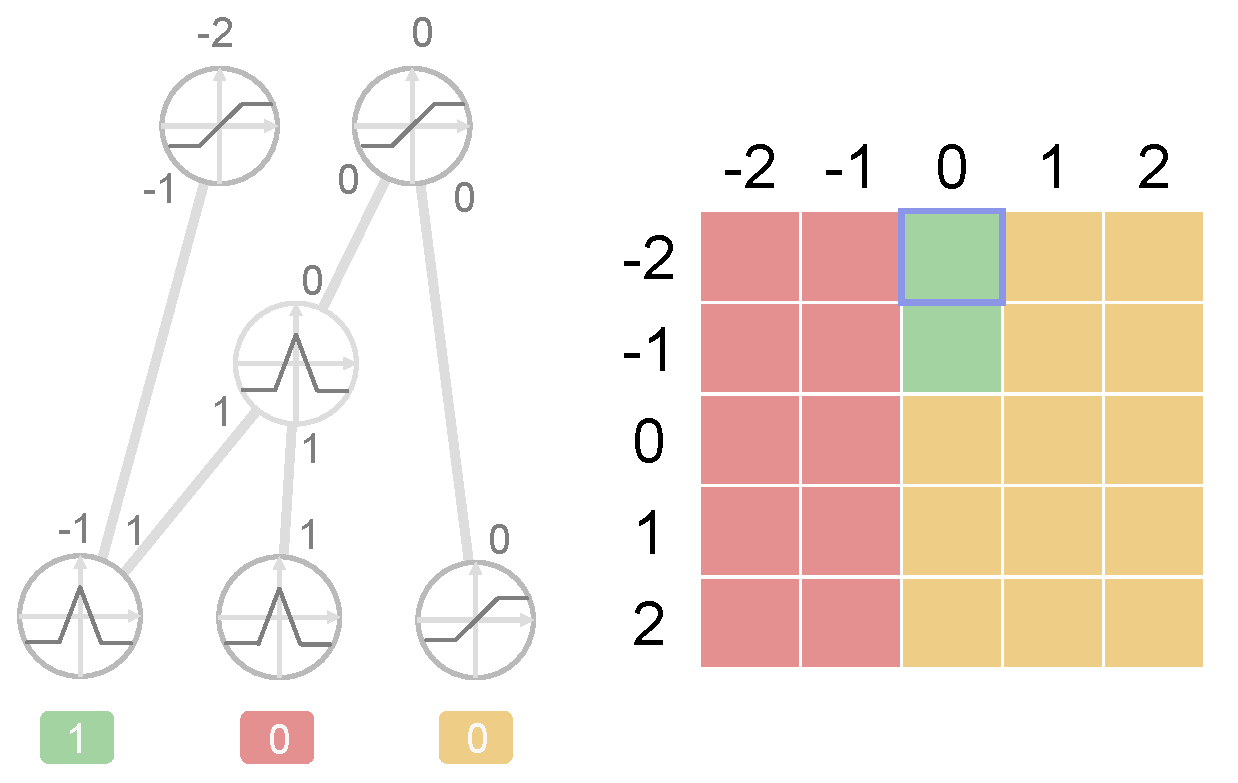
\includegraphics[width=\textwidth]{figure/CPPN2}
  \caption{
  Example of a compositional pattern-producing network. Input is z and y coordinates. The actual simulation model also uses the z-coordinate as well as r, the radial distance to origo, but they are for the sake clarity not included here. For the same reason all links have the weight of one. The pattern seen on the right is the result of evaluating the network seen on the left. The currently evaluated cell \((-2,0)\) is marked with a blue border and is coloured green since the output node corresponding to the green colour has the highest output value. Numbers above the nodes are their input values while the numbers above are their output.
  }
  \label{fig:cppn} 
\end{figure}

\subsection{Neuroevolution of Augmenting
Topologies} \label{subsec:NEAT}
NeuroEvolution of Augmenting Topologies (NEAT) is a method presented by \cite{stanley2002evolving} where not only the edge weights of a network, but also the network topology is evolved over time. This is done in order to avoid fixing the network structure beforehand. 

In this model, mutations suggested by \cite{stanley2002evolving} and \cite{stanley2007compositional} are used, but crossover is disregarded since the organisms only reproduce asexually. While crossover could possibly improve the evolution of the organisms, its implementation was left outside the scope of this project.

\begin{description}
    \item[Mutate weights] With a certain mutation probability, each node is perturbed by a certain amount
    \item[Add node] A hidden node is added at the site of a current connection, replacing the connection and creating new connections to the previously connected nodes
    \item[Add connection] A new connection is added between two random nodes. However there can be no connections going into input or bias nodes nor any out of output nodes.
    \item[Remove connection] A random connection is removed. If this causes a hidden node to be without any connections, that node will be removed as well.
\end{description}

\subsection{Genotype to phenotype mapping}\label{subsec:genToPhenMapping}
In the genome network implemented for the final long-term simulation (described in the results chapter \ref{cpt:Results}), there are four input nodes. Together they specify the initial distance and position of the current cell relative to the organism origin. Furthermore, there are nine output nodes: one for each cell type, plus one extra output node determining the cell radius. The node indices are assigned as follows:
\begin{description}
\item[Input nodes]{\scriptsize
    \begin{tabular}{ | c | c | c | c |}
      0 & 1 & 2 & 3 \\
      x & y & z & r \\
    \end{tabular}}
\item[Output nodes]{\scriptsize
    \begin{tabular}{| c | c | c | c | c | c | c | c || c | c | c |}
     4 & 5 & 6 & 7 & 8 & 9 & 10 & 11 & 12 & 13 & 14 \\
    Photo & Digest & Sting & Vascular & Fat & Sense & Egg & Buoyancy & Cell radius & &  \\
    \end{tabular}}
\item[Bias nodes]{\scriptsize
    \begin{tabular}{| c |}
      15 \\
      Gives constant value of 1 \\
    \end{tabular}}
\item[Hidden nodes]{\scriptsize
    \begin{tabular}{| c |}
     16 and onward
    \end{tabular}}
\end{description}
In order to determine the cell type, the output nodes 4 through 11 are inspected. The cell type corresponding to the output node with the largest value will be selected. Compare this with the example of the colored lattice in Figure \ref{fig:cppn}.

If two values are exactly equal, preference will be given to the lower node id. However, if no node produces a value over 0 the cell will not be created at all. Of the nodes 12, 13 and 14 only the node 12 fills a purpose. The remaining two were actually left as a mistake in the initial organism genome from earlier versions of the model, where the density and other properties of cells were also considered for genome output.

\section{Definition of an organism}
An organism is modelled to consist of three parts:
\begin{enumerate}
    \item The genome, a genotype-to-phenotype mapping structured as a CPPN (see subsection \ref{subsec:CPPN})
    \item The nervous system, an artificial neural network to allow the organism to interact with it's surrounding
    \item A list of the particles that constitutes its cells.
\end{enumerate}
Each cell has a link to its von Neuman neighbours, so that each pair of neighbour particles can exert a spring force holding the organism together.

\tempText{Note that there is a cost for large network sizes}

\subsection{Genome}
The genome consists of a CPPN, as described in \ref{subsec:CPPN}, as well as a discrete vector of organism diameters \(\mathbf{D_{org}}=\left(\begin{array}{ccc} d_x & d_y & d_z \\\end{array}\right)\). An organism consists of at least one cell, placed at the origin, while \(\mathbf{D_{org}}\) determines the number of cells outside of it in each direction. Thus, the size of the resulting rectangular cuboid of cells is
\(\mathbf{S_{org}}=\left(\begin{array}{ccc} 2 d_x + 1 & 2 d_y + 1 & 2 d_z + 1 \\\end{array}\right)\).

Given the cell index as input to the CPPN, the resulting output determines the cell type (as well as optional cell properties, for example radius or density), thus defining the organism phenotype.

When an organism reproduces, its genome (and nervous system) will mutate as it is copied to the offspring. The CPPN will mutate according to the NEAT method described in \ref{subsec:NEAT}, while \(\mathbf{D_{org}}\) might increase or decrease in either of its vector components.

\subsection{Nervous system} \label{subsec:nervousSystem}
The nervous system is an ANN (artificial neural network) very similar in structure to the CPPN in the genome and also evolved using the NEAT method (described in \ref{subsec:NEAT}). The input to the nervous system consists of signals from the sensor cells as well as from a bias node sending out a constant value of 1. The output consists of a movement vector for the organism in its local coordinate system, converted to the global coordinate system as described in section \ref{sec:orgCoordSys}.

\section{Organism coordinate system}\label{sec:orgCoordSys}
The most simple approach for generating movement from the output of the nervous system would be to directly output a force vector \(f=\left(\begin{array}{ccc} f_x & f_y & f_z \\\end{array}\right)\) in the global coordinate system, where the three components of \(f\) are the three output values from the network and \(f\) is added to the current total force of the organism.

However, this approach creates an inherent knowledge of world direction, easily causing the organisms to move, for example: directly up, north or west. As such, the organism in this model instead moves according to their local coordinate system, an approach which will be explained in this section.

\begin{figure}
  \centering
  \includegraphics[width=0.6\textwidth]{figure/neighbours}
  \caption{Identifiers for the six three-dimensional von Neumann neighbours to a cell. Subscripts denote distance in x, y, and z directions between the cell and each neighbour at birth.}
  \label{fig:neighbours} 
\end{figure}

The organisms does not have any stored orientation, since they still consists of relatively independent cells. However, cells have links to their 3-dimensional von Neumann neighbours; front, back, left, right, up and down. These are denoted \(n_{x,y,z}\) as in Figure \ref{fig:neighbours}, where x, y and z are initial distances between the neighbouring cells.

For each neighbour \(n_{x,y,z}\), we then calculate a vector \(v_{x,y,z}\) pointing in their direction as follows:
\[
v_{x,y,z} = 
\begin{cases}
pos(self) - pos(n_{x,y,z}), & \text{if }n_{x,y,z} \text{exists}\\
(0,0,0), & \text{otherwise}
\end{cases}
\]
The function \(pos(n)\) gives the current position of the neighbour \(n\).
Cells at the edges of an organism does not have any neighbours in their "outward" directions, so a zero vector is returned from \(v_{x,y,z}\) if the neighbour does not exist. 

A property of the neighbourhood structure is that the top and bottom neighbour vectors, for example, should point in almost opposite directions. Thus, the six vectors \(v_{0,0,1}, v_{0,0,-1}, ..., v_{-1,0,0}\) can be reduced to three by taking the sum of the linearly dependent pairs:
\begin{align*}
v_x = v_{1,0,0} - v_{-1,0,0}\\
v_y = v_{0,1,0} - v_{0,-1,0}\\
v_z = v_{0,0,1} - v_{0,0,-1}
\end{align*}

These three vectors would work as base vectors defining the local coordinate system of the cell. However, to further account for missing neighbours, each is also combined with the cross product of the other two. Normalised and written as the columns of the transformation matrix \(\mathbb{M}\) we get:

\[
\mathbb{M}=
\left(
\begin{matrix}
 norm(v_x + (v_y \times v_z)), &&
 norm(v_y + (v_z \times v_x)), &&
 norm(v_z + (v_x \times v_y))
\end{matrix}
\right)
\]

Where \(norm(v) = \frac{v}{|v|}\).

Thus from the movement force \(f_{local}\) given by the nervous system in the local coordinate system, we get the force to be applied onto the cell in global coordinates as \(f_{global} = 
c_{move}(\mathbb{M} \cdot f_{local} ) \), where \(c_{move}\) is a movement parameter.

\section{The energy cycle}\label{sec:EnergyCycle}
The final part of the model to be explained here is the energy cycle; how the energy is transferred through the system.

Each photosynthetic cell is paired with an energy particle. The energy particle is initialised just above the cell and travels straight upwards with a speed of one particle diameter per timestep. Each timestep the cell gains an amount of energy proportional to its cross-section area, provided that the energy particle reaches the top of the simulated volume without any collisions. If there is a collision, the cell will stop gaining energy until the view is once again clear. When the particle reaches the top of the volume it is returned to a position just above the cell. Figure \ref{fig:energyParticles} illustrates this with an example of photosynthetic cells and their respective energy particles.

\begin{figure}
  \begin{center}
  \includegraphics[width=\textwidth]{figure/energyParticles}
  \caption{
    Energy particles rising from an early population of photosynthetic organisms. Each energy particle belongs to a photosynthetic cell. If the energy particle reaches the top of the arena without colliding with any cells, the photosynthetic cell it belongs to will continue gaining energy every frame. If the particle does collide, the cell will not get any energy until its particle once again can complete the distance without collisions. In this illustration, energy particles that have collided are coloured blue, while the rest are red. The cells are opaque and coloured according to the amount of energy they contain, with warm colours indicating higher energy density.  
  }
  \label{fig:energyParticles}
  \end{center}
\end{figure}

Digestive cells and sting cells are the other two cell types that harvest energy to an organism, as described in subsection \ref{subsec:cellTypes}. From them and the photosynthetic cells, the energy is dispersed within the organism. Different cell types disperse energy in different amounts. For example, egg cells only absorb energy without ever giving anything back, while the energy-harvesting cells part with most of their energy. See Table \ref{tab:cellEnergies} for an example of how the energy dispersion was configured in the final run described in the results.

\begin{table}[H]
 \begin{tabular}{| c || c | c | c|} 
    \hline
     Cell type & Energy in & Energy out & Maximum energy \\ [0.5ex] 
     \hline\hline
     Photosynthetic & 0.01 & 0.5 & 10 \\ \hline
     Digestive & 0.01 & 0.5 & 10 \\ \hline
     Sting & 0.01 & 0.5 & 10 \\ \hline
     Vascular & 1 & 0.2 & 3 \\ \hline
     Fat & 1 & 0.01 & 50 \\ \hline
     Sensor & 1 & 0 & 5 \\ \hline
     Buoyancy & 1 & 0 & 5 \\ \hline
     Egg & 1 & 0 & 1000 \\ \hline
 \end{tabular}
\caption{Example of a cell types energy configuration. \emph{Energy in} is the portion of the energy offered by a neighbour that is absorbed,  \emph{Energy out} is the the portion of the cell's surplus energy that is offered to a neighbour.}
\label{tab:cellEnergies}
\end{table}